\documentclass{article}
\usepackage[T1]{fontenc}
\usepackage{lmodern}
\usepackage{graphicx}
\usepackage{amsmath,amssymb}
\usepackage[a4paper,margin=2cm]{geometry}
\usepackage[absolute,overlay]{textpos}
\setlength{\TPHorizModule}{1mm}
\setlength{\TPVertModule}{1mm}
\usepackage[indonesian]{babel}
\usepackage{hyperref}
\setlength{\emergencystretch}{2em}
% unit: Halaman 23

\begin{document}

% === Halaman 23 (llm) ===

\vspace{135.73mm}

Contoh 3: \[ a \cdot b = (x^3 + x^2 + 1) \cdot (x^2 + x) = x^5 + 2x^4 + x^3 + x^2 + x \pmod 2) \\ = x^5 + x^3 + x^2 + x = 10110 \]

% deskripsi: Proses pembagian polinomial untuk mencari sisa pembagian (modulo) dari x^5 + x^3 + x^2 + x oleh x^4 + x + 1
% bbox normalisasi: [0.1800, 0.2400, 0.6070, 0.6970]
\begin{textblock*}{89.67mm}(37.80mm,71.28mm)
\noindent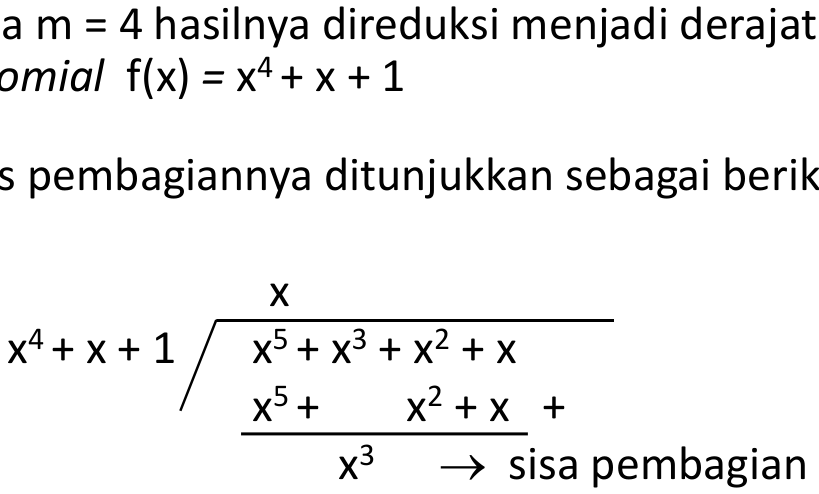
\includegraphics[width=89.67mm,height=135.73mm]{../../images/llm/page_023_img_01.png}%
\end{textblock*}

\end{document}
